\chapter{Results}\label{sec:results}

\section{Experiments}\label{sec:experiments}

As already mentioned in the beginning we were interested in two qualities of our system. Most importantly, we wanted to find out what advantages the speed gain with the DVS would provide for quadcopter tracking. An already proven advantage is the opportunity to track active markers.  This is beneficial for searching trackable features as they are easier to identify and thus faster to find. In order to test these performance properties of our algorithm a suitable experimental setup needed to be designed. To measure how fast our system would perform under conditions where convetional cameras tend to fail, we planned to test it under real conditions by flying aggressive maneuvers with a quadcopter. Furthermore, since the DVS has a much lower resolution than today's standard CMOS cameras, the accuracy at which pose can be estimated with the DVS needed to be evaluated as well. \cite{Saner} has developed a framework for controlling the ARDrone including the ability to let the drone execute a flip, i.e. a 360\degree roll. We decided to use this flip as our aggressive maneuver. We would then measure the time interval during which tracking was lost.


\begin{figure}[h]
     \centering
     \includegraphics[height=0.5\textwidth]{img/marked_quadrotor.jpg}
     \caption{The ARDrone 2.0 equipped with reflecting markers and LEDs.}
     \label{img:marked_quadrotor}
\end{figure}

\subsection{Setup}\label{sec:experimentalsetup}

For our setup we used the commercially available ARDrone 2.0 (Figure \ref{img:marked_quadrotor}) on which we attached our active markers as well as the microcontroller. Each LED was fixed facing downwards (if one assumes the drone to be in steady flight mode), one under each of the four rotors (Figure \ref{img:quadcopter_belly}). All four LEDs where lying on a plane forming a square with 20cm side length. The USB connector available on the drone provided power to the microcontroller and LEDs. For tracking the quadcopter, the DVS was installed on the floor facing upwards (Figure \ref{img:dvs_ground}).

\begin{figure}[h]
     \centering
     \includegraphics[height=0.5\textwidth]{img/quadcopter_belly.jpg}
     \caption{The underbelly of the quadcopter. The circles indicate the LED positions.}
     \label{img:quadcopter_belly}
\end{figure}

\begin{figure}[h]
     \centering
     \includegraphics[height=0.5\textwidth]{img/dvs_ground.jpg}
     \caption{DVS setup for data recording.}
     \label{img:dvs_ground}
\end{figure}


\subsubsection{Tracking speed comparison}\label{sec:trackingspeedcomparison}

In order to be able to compare the performance of the DVS to a conventional camera, we used the onboard front-looking camera on the quadcopter. The image data was streamed to a computer via network interface, were the parallel tracking and mapping algorithm (PTAM)\cite{PTAM} was employed for pose estimation.


\subsubsection{Pose estimation accuracy}\label{sec:poseaccuracy}

To measure the pose estimation accuracy we needed a reference. For this task we used the OptiTrack from NaturalPoint\footnote{http://www.naturalpoint.com/optitrack/} which is a marker-based optical motion tracking system. It offers millimeter accuracy and was thus a very good approximation to the real positon. Four markers have been applied to the drone in order to make it trackable with the OptiTrack.

\subsubsection{Data recording}\label{sec:datarecording}

Using this setup we did several recordings, where the position data from the OptiTrack, the image data and pose from the drone's onboard camera, as well as the raw event data from the DVS were recorded. We used the robot operation system\footnote{http://www.ros.org} (ROS) for this purpose.
As the data came from different systems we needed a way to synchronize the measurements afterwards. We decided to use a motion induced cue for synchronization by moving the drone up and down by hand, generating a sinusoid curve in the position data. This was later used for manual time synchronization of the recordings. 
Each recording then started with inducing the cue followed by the drone being remotely piloted to fly over the DVS camera where we would trigger a sideway flip. 


\subsubsection{Difficulties}\label{sec:difficulties}

During the recordings we met a number of unforeseen difficulties. Having attached the LEDs and microcontroller to the drone we found that it had become unstable during flight and hard to control remotely. Although the drone's motors are powerful enough to pull it upwards it had obviously not been designed with additional payload in mind. Another problem of the additional payload was that the drone was not able to output enough power to keep a stable height after the flip. Instead it usually came crashing down onto the floor. This meant that a stable reacquisition of the localization with the drone's internal camera had a higher latency than expected. 
The optical tracking system introduced another challenge into the experiments, since it uses reflecting markers for tracking which illuminated by high-power infrared spotlights. In the OptiTracks standard setup, the spotlights are pulsed. The DVS is very sensitive to the infrared spectrum and, as we found, the strobing generated a buffer overflow on the DVS as it could not the high amount of events arriving at the same time. Therefore it was paramount to deactivate the strobing for all the cameras prior to recording. Also, the infrared illumination from the OptiTrack seemed to impede the sensitivity towards our LEDs, although this barely influenced our experiment setup.


\section{Evaluation}\label{sec:evaluation}

Due to the above difficulties out of 18 executed flips only 6 had feasible data. In the following two paragraphs the measurements of tracking downtime, as well as the pose estimation accuracy are discussed. Before evaluation the data from the DVS had yet to be passed through our algorithm. 


\subsection{Tracking speed}\label{sec:trackingspeed}

To measure how fast the different systems are able to reacquire tracking we first synchronized the recordings by hand. As during the recordings the DVS lost track of the LEDs on several occasions, due to them being out of view, the interval during which a flip happened, as well as the time measurements needed to be taken manually. The time for a flip was measured by considering the roll data from the OptiTrack, taking the interval between the last measurement before the flip and the first measurement after the flip where the helicopter was in a level orientation to the floor. To measure the onset and offset of losing tracking on the DVS, the last sample before losing track (i.e.  where the interval position samples were considerably higher than the mean sampling rate) and the first sample of reacquiring track (regaining a steady sample rate).  The same was done for the PTAM data. Unfortunately, as previously mentioned, the helicopter usually crashed into the floor after doing a flip. Therefore there often was no stable position data for several seconds. Nevertheless, few single samples with reasonable positioning were recorded before crashing which were thus taken as a reference. Figure \ref{img:fliptimes} shows a statistical comparison of the time intervals in which the different approaches lost tracking compared to the duration of flips. The red bar indicates the median while the blue box marks the first and third quartile. The whiskers extend to a range of 1.5 times the range between the first and third quartiles. All data points outside this range are considered outliers and are marked with a red plus. 
Table \ref{tab:downtime_tab} shows the mean standard deviation of the different approaches. Our algorithm lost track during the average time of 0.35 seconds. PTAM respectively lost track for a mean of 0.8 seconds which is more than twice the time of the DVS and takes longer than the average duration of a flip. One can clearly see that the time where tracking is lost is much shorter with our approach in respect to PTAM. As figure \ref{img:mean_downtime} further illustrates, the downtime for the DVS stays inside the interval of the flip duration. The results emphasize that the DVS is faster in recovering lost tracks than the PTAM approach. As verified with our recordings, the downtimes  of the DVS correspond to losing sight of the LED markers because of their emission angle. In contrary to PTAM tracking on the DVS is lost due to the marker configuration rather than fast motion. We reckon that with a suitable configuration of either more markers or dynamic vision sensors, tracking could be maintained during the whole flip. PTAM shows to lose track for a longer duration than the flip takes. In contrary to the DVS the the camera of the drone loses sight of its tracked features due to blurring in the camera image and thus takes a longer time to recover.

\begin{table}\label{tab:downtime_tab}
	\centering
    \begin{tabular}{|l|l|l|}
        \hline
        ~    & \overline{x}\ [s]   &    \sigma\ [s]     \\ \hline
        DVS  & 0.35   &   0.10 \\ 
        PTAM & 0.80   &  0.33 \\ 
        Flip & 0.56   &   0.15 \\
        \hline
    \end{tabular}
	\caption{Mean and standard deviation of tracking downtime intervals and the flip duration.}
\end{table}

\begin{figure}[h]
     \centering
     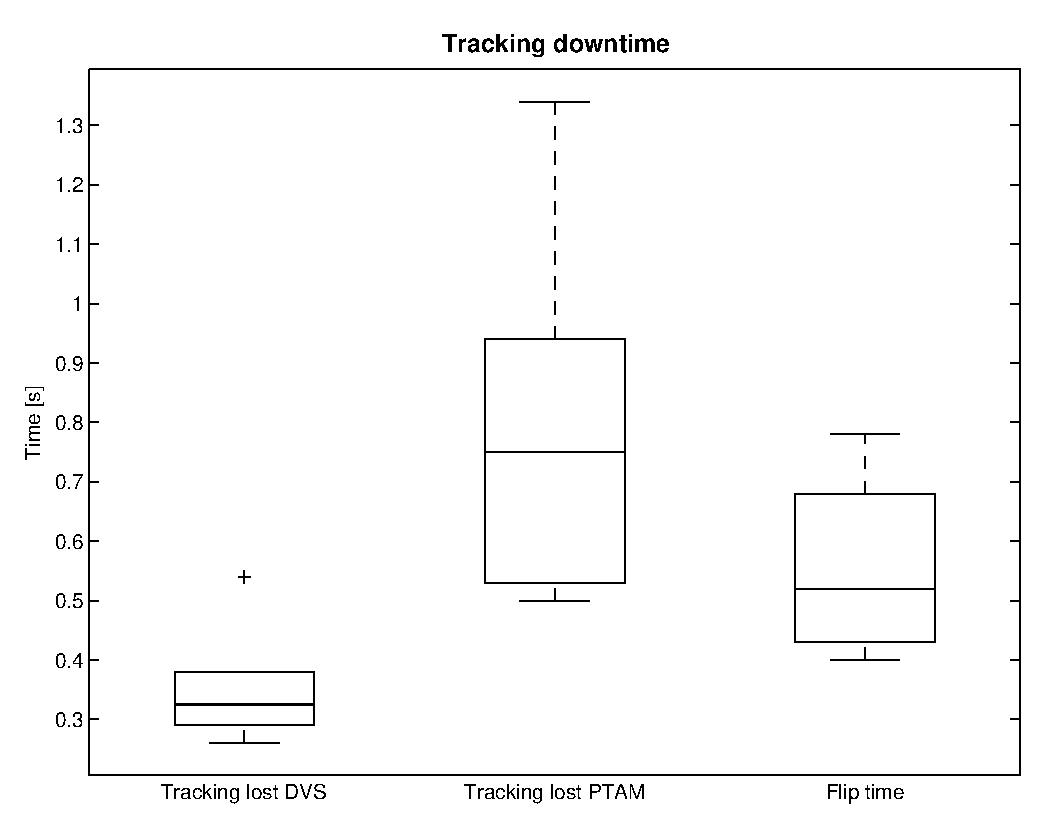
\includegraphics[width=1.0\textwidth]{img/flip_times.eps}
     \caption{Statistical plot of measure time interval. The boxplots show the time interval in which tracking is lost for the our algorithm and PTAM compared to the duration of a flip.}
     \label{img:fliptimes}
\end{figure}

\begin{figure}[h]
     \centering
     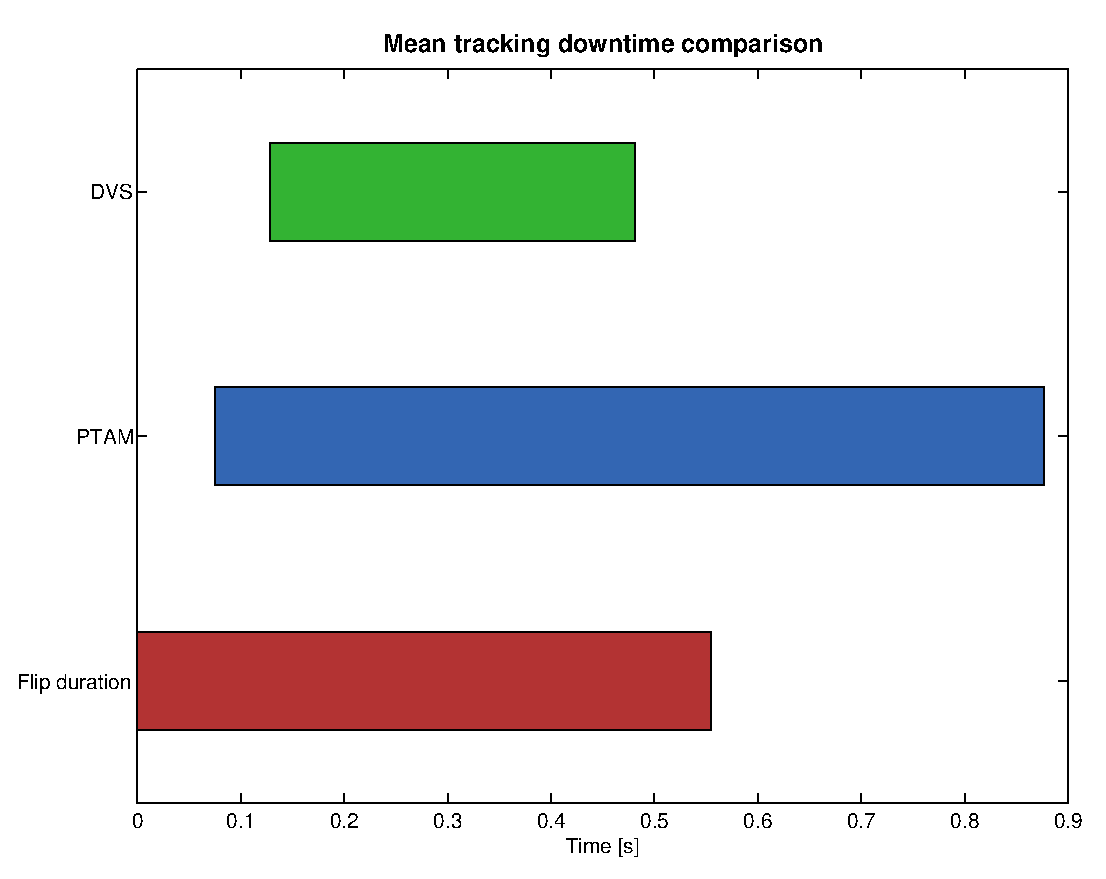
\includegraphics[height=0.5\textwidth]{img/mean_flip_times.eps}
     \caption{Comparison of the mean tracking downtime intervals. The mean time intervals of both algorithms are compared against the mean flip time on a time line.}
     \label{img:mean_downtime}
\end{figure}

\subsection{Pose estimation}\label{sec:poseestimationeval}

In order to measure the accuracy of pose estimation from the DVS the OptiTrack data was used as a reference. Apart from synchronizing the measurements in time we also needed to align the different reference frames from the DVS and OptiTrack system first. This was achieved using equation \ref{eq:leastsquares} to find the correct transformation \{\emph{R},\emph{t}\}.
 
 \begin{equation}\label{eq:leastsquares}
      \begin{aligned}
        \sigma = \min_{R,t} \sum_{i} ( {S_{i} - (R T_{i} + t))^2\ \text{with}\ S,T \in \mathbb{R}^3.\\
      \end{aligned}
 \end{equation}

Before doing so the data sets were first brought to the same number of samples with a common time stamps. As the DVS has a lower sampling rate than the OptiTrack the OptiTrack data was resampled by linearly interpolating the translation and rotation. The transformation gained from the least-squares algorithm was then used to align the OptiTrack coordinate system to the one from the DVS. Last, the absolute errors were taken from the translation data. The rotation data, expressed in roll pitch and yaw, was again fitted from the OptiTrack to the DVS frame according to the least-square error. The same analysis was done on the PTAM data in order to compare the two approaches in their accuracy. Table \ref{tab:trans_error_tab} shows the mean and standard error for the translation in both approaches. The DVS' average error is roughly two times lower than PTAM. Figure \ref{img:trans_error_box} shows the statistical distribution of the pose errors ( for details on the boxplot, please refer to \ref{sec:trackingspeed}). Although the spread of outliers is higher in our approach compared to PTAM, the translation errors of the latter technique show a broader distribution around their median. Overall this proves the DVS approach to have a higher accuracy with less spread if neglecting the outliers. Figures \ref{img:roll_error_box},\ref{img:pitch_error_box} and \ref{img:yaw_error_box} display the error distribution for roll, pitch and yaw respectively. The DVS performs worse in roll and pitch compared to yaw. This was to expect, due to the oscillating LED position as described in section \ref{sec:approach_discussion}, position estimations in depth have less accuracy. As roll and pitch play a minor roll in qaudrotor pose estimation these can be neglected for finding the drone's orientaion. Table \ref{tab:yaw_error_tab} demonstrates that the DVS performs slightly worse than PTAM with a mean error of 6 degrees and a deviation of 15 degrees. 

\begin{table}\label{tab:trans_error_tab}
	\centering
    \begin{tabular}{|l|l|l|}
        \hline
        ~    & \overline{x}\ [cm]   &    \sigma\ [cm]     \\ \hline
        DVS  & 8.9   &   12.6 \\ 
        PTAM & 19   &  12.4 \\ 
        \hline
    \end{tabular}
	\caption{Mean and standard deviation of translation error of the DVS and PTAM.}
\end{table}

\begin{table}\label{tab:roll_error_tab}
	\centering
    \begin{tabular}{|l|l|l|}
        \hline
        ~    & \overline{x}\ [^{\circ}]   &    \sigma\ [^{\circ}]     \\ \hline
        DVS  & 19   &   27 \\ 
        PTAM & 7   &  22 \\ 
        \hline
    \end{tabular}
	\caption{Mean and standard deviation of roll error of the DVS and PTAM.}
\end{table}

\begin{table}\label{tab:pitch_error_tab}
	\centering
    \begin{tabular}{|l|l|l|}
        \hline
        ~    & \overline{x}\ [^{\circ}]   &    \sigma\ [^{\circ}]     \\ \hline
        DVS  & 17   &   18 \\ 
        PTAM & 5   &  11 \\ 
        \hline
    \end{tabular}
	\caption{Mean and standard deviation of pitch error of the DVS and PTAM.}
\end{table}

\begin{table}\label{tab:yaw_error_tab}
	\centering
    \begin{tabular}{|l|l|l|}
        \hline
        ~    & \overline{x}\ [^{\circ}]   &    \sigma\ [^{\circ}]     \\ \hline
        DVS  & 6   &   15 \\ 
        PTAM & 3   &  10 \\ 
        \hline
    \end{tabular}
	\caption{Mean and standard deviation of yaw error of the DVS and PTAM.}
\end{table}

\begin{figure}[h]
     \centering
     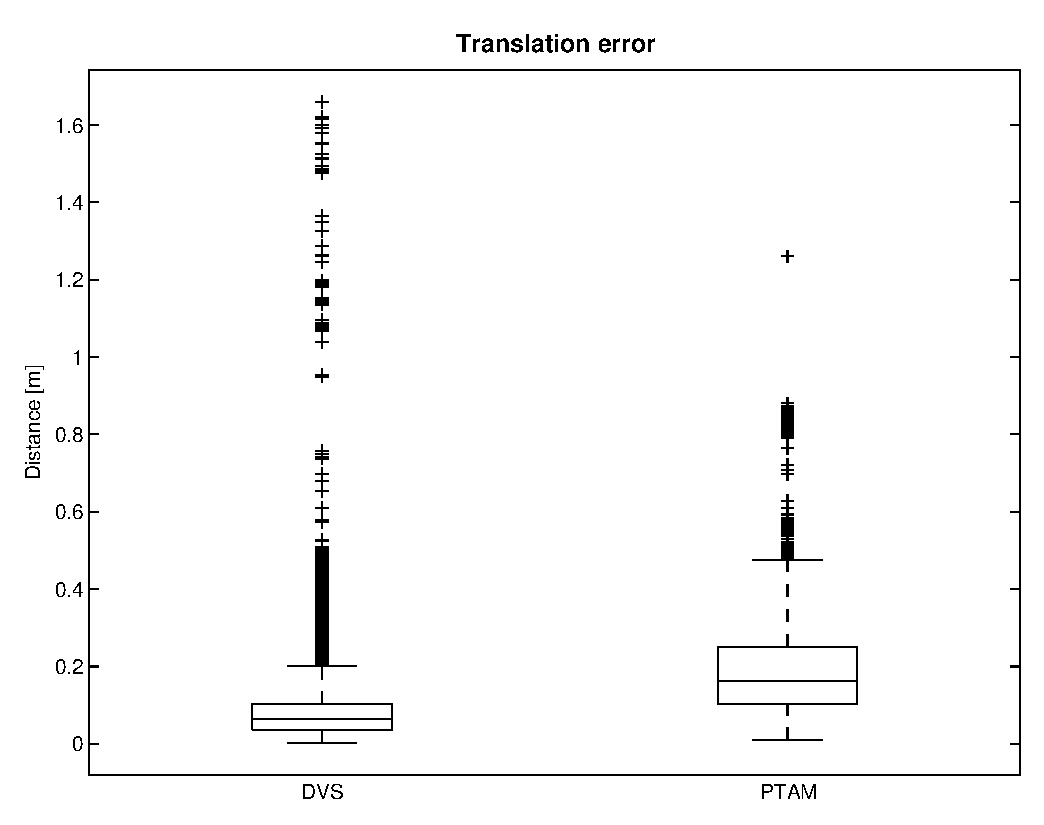
\includegraphics[width=1.0\textwidth]{img/trans_error_box.eps}
     \caption{Statistical plot of the pose estimation error of the DVS in reference to the OptiTrack measurements.}
     \label{img:trans_error_box}
\end{figure}

\begin{figure}[h]
     \centering
     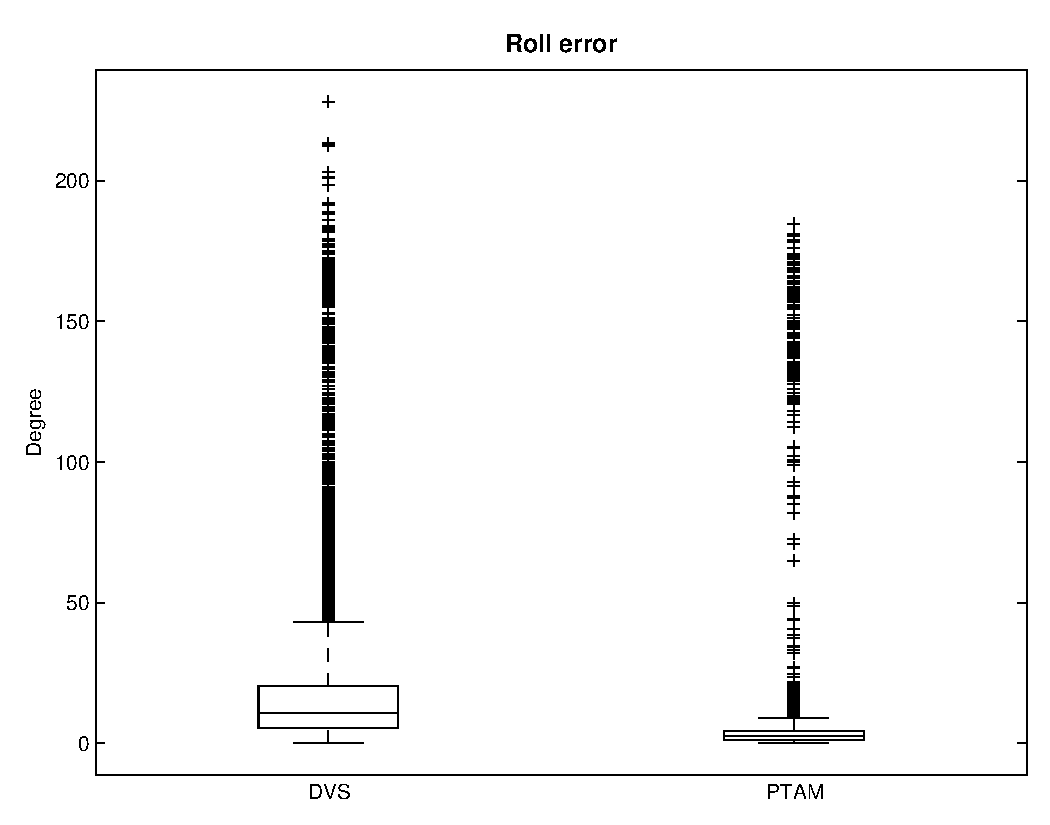
\includegraphics[width=1.0\textwidth]{img/roll_error_box.eps}
     \caption{Statistical plot of the rotation error of the DVS in reference to the OptiTrack measurements.}
     \label{img:roll_error_box}
\end{figure}

\begin{figure}[h]
     \centering
     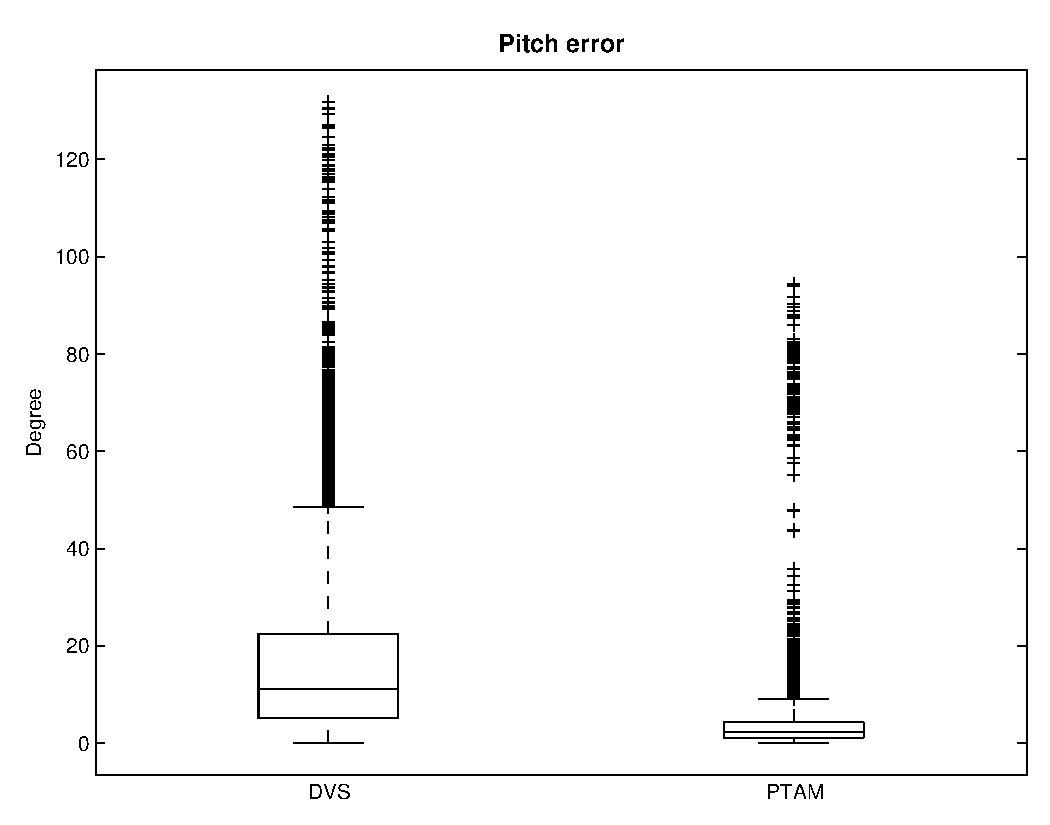
\includegraphics[width=1.0\textwidth]{img/pitch_error_box.eps}
     \caption{Statistical plot of the pose estimation error of PTAM in reference to the OptiTrack measurements.}
     \label{img:pitch_error_box}
\end{figure}

\begin{figure}[h]
     \centering
     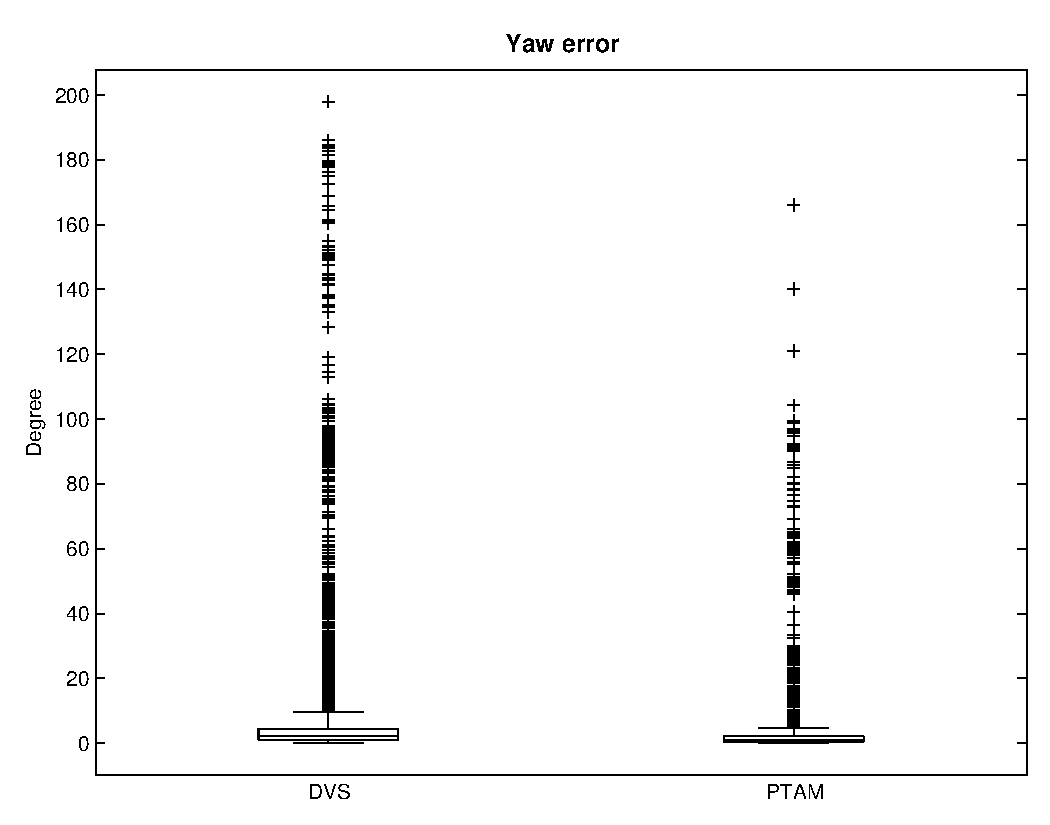
\includegraphics[width=1.0\textwidth]{img/yaw_error_box.eps}
     \caption{Statistical plot of the rotation error of PTAM in reference to the OptiTrack measurements.}
     \label{img:yaw_error_box}
\end{figure}


\section{Discussion}\label{sec:eval_discussion}

Overall the pose estimation for the DVS provides good results compared to PTAM. While the translation estimation with the DVS has a clear advantage, the rotation error is less accurate. The oscillating position information of LEDs seems to have a higher influence on the rotation estimation compared to translation. Improving the algorithm to provide more stable marker tracking is thus an important starting point to improve the overall accuracy.